\documentclass[a4paper, 12pt, titlepage]{article}
\usepackage{listings,amssymb, amsmath, amsthm, graphicx, float}
\author{Joris Stork: 6185320 \and Lucas Swartsenburg: 6174388 \and Sander van
Veen: 6167969}
\title{Laboratory log book Robotics}
\begin{document}
\maketitle
\tableofcontents 

\newpage

\section{I$^2$C and the CSS Compiler} % {{{

\subsection{Objective} % {{{

Our objective is to implement an I$^2$C bus using: a 3-state word generator, an
I/O expander and a microcontroller (these are described below). 
The I$^2$C bus is a two-wire serial bus used for data transport between
integrated circuits.

% }}}

\subsection{Method} % {{{
Our implementation of the I$^2$C bus involves transporting 8 parallel bits of data -
generated by a human operator via the interface of a word generator -
over from the I/O expander using the 2 bit I$^2$C protocol to the microcontroller, and
back again. We programmed the
microcontroller in a C-like language and used the provided C API (functions
\texttt{i2c\_read} and \texttt{i2c\_write}) to act as the master on the I$^2$C
bus, with the I/O expander as slave (see the appendix for code). 
We connected the microcontroller's C4 and C3 pins with the I/O expander's
SDA (serial data line) and SCL (serial clock line) pins respectively. The I/O
expander's eight left-hand side pins were connected to the corresponding eight
pins of the word generator.
The program loaded onto the microcontroller initiates the transfer on the bus,
first setting the SDA signal to ``low'', then  
indicating the transmission direction (from slave to master) and the address of
the slave (corresponding to the left-hand pins of the I/O expander) from which
to send the data. Once the microcontroller had received the data, the program
initiated a second transfer in the opposite direction, sending the same data it
had received back to the I/O expander for display on the I/O expander's
right-hand LEDs.

% }}}

\subsubsection{Hardware}

\begin{itemize}
\item PCF8574 I$^2$C I/O expander integrated circuit (IC).
Each of this I/O expander's eight pins can be used as an input or output. In order 
to use a pin as input, a 1 has to be written to that pin's register.
\item 16F876 microcontroller: this is an 8 bit microcontroller that we load with
programs written in mplab \dots
\item 74LS244 word (8 bit) generator. Buttons toggle each of the eight pins
representing the 8 bits of output.
\end{itemize}

\subsubsection{Software}
The follows software runs on an i86 Windows XP machine which is connected to the
microcontroller using a serial port cable.
\begin{itemize}
\item Tera Term Web 3.1 : used as a terminal console for the microcontroller.
\item MPLAB IDE v6.30
\item PIDAC 876 programmer: Loads the compiled program onto the microcontroller
using the serial port.
\end{itemize}

% }}}

% }}}

\subsection{results} % {{{
The experiment worked as expected. The \texttt{0b11000110} was transmitted and
returned successfully, as shown in the image below:
\begin{figure}[H]
\caption{Photo set-up$I^{2}C$}
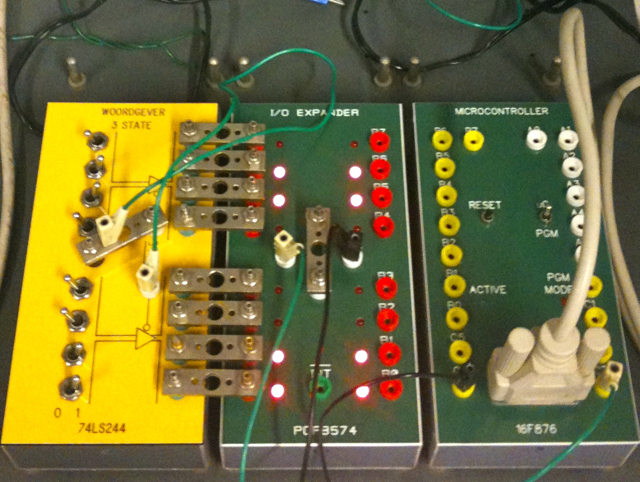
\includegraphics[scale=0.61]{IMG_0703}
\end{figure}

\begin{figure}[H]
\caption{Diagram set-up $I^{2}C$}
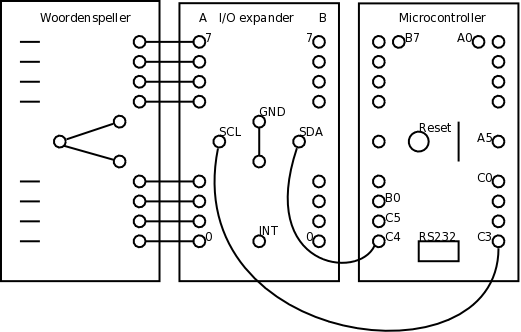
\includegraphics[scale=0.61]{I2C.png}
\end{figure}

% }}}

\subsection{assumptions} % {{{

We didn't make any assumptions, so nothing useful to mention here.
% }}}
\newpage
\section{SAR ADC} % {{{

\subsection{Objective} % {{{
Our objective is to convert a analog signal to a digital signal and 
to test how accurate and what the range of our equipment is. We also wan't to find out what the relation is between the voltage and the digital value that is produced. This experiment is in preparation of the next one. \\
\\
In this experiment we assume that the relation between the voltage and the digital value is 0.40v/bit because that is what is written on the outside of the equipment.
assume t
% }}}

\subsection{Method} % {{{

We attach a SAR (successi­ve approxima­ti­on register) to the comperator. The SAR will conduct the comparator so that the current voltage can be found with a binary search. The results of the comparing operation will be written to a I/O expander. It wasn't part of this assignment, but (like shown in the previous assignment) it is possible to attach the I/O expander using a $I^{2}C$ bus to a microcontroller. This way we can read out the values on the computer screen. The potentiometer has 10 positions. We shall test the voltage and digital value on each position.

% }}}

\subsection{Equipment} % {{{
\subsubsection{Hardware}

\begin{itemize}
\item PCF8574 I$^2$C I/O expander integrated circuit (IC).
\item 4 bit Value generator. 
\item Pulse generator (clock). We used one wich had different frequencies, but we liked using the 1Mhz clock.
\item SAR (successi­ve approxima­ti­on register). A SAR is a IC that conducts succesive approximation using a comperator.
\item Comperator. The comperator also has a digital to analog converter on board. The SAR gives a digital signal to the comperator and the comperator produces a currancy. This currancy is compared to the currancy on the input of the comperator. If the analog input currancy is higher than the produced currancy, the comperator will return a 1 to the SAR. Otherwise, a 0.
\item Potentiometer. On the potentiometer there are 11 spots, marked from 0 to 10. On each of these spots the potentiometer will give a certain currance. This currancy will grow exponetially going from 0 to 10. 
\item A voltage meter. We used a voltage meter to measure the currancy coming the potentiometer. Its purpuse in this setup is to check the relation between the digital signal from the SAR and the voltage.
\item (Optional) 16F876 microcontroller: this is an 8 bit microcontroller that we load with
programs written in mplab \dots
\end{itemize}

\subsubsection{Software}
For this assignment we don't need to use any software. Only when we want to read out the digital values on a computer screen, we can use the code of the previous assignment ($I^{2}C$).
\begin{itemize}
\item Tera Term Web 3.1 : used as a terminal console for the microcontroller.
\item MPLAB IDE v6.30
\item PIDAC 876 programmer: Loads the compiled program onto the microcontroller
using the serial port.
\end{itemize}
% }}}

\subsection{Raw results} % {{{


\begin{table}[H]
\centering
\begin{tabular}{|l|l|l|l|l|} \hline
Potentiometer & Voltage (Volt) & Binary & Decimal & Value / Voltage\\ \hline
 0 & 0.00 & 0000 0000 & 0 & 0.0000 \\ \hline
 1 & 0.02 & 0000 0001 & 1 & 0.0200 \\ \hline
 2 & 0.09 & 0000 0010 & 2 & 0.0450 \\ \hline
 3 & 0.29 & 0000 0011 & 3 & 0.0966 \\ \hline
 4 & 0.52 & 0000 0110 & 6 & 0.0866 \\ \hline
 5 & 0.74 & 0000 1111 & 15 & 0.0493 \\ \hline
 6 & 0.98 & 0001 1000 & 24 & 0.0408 \\ \hline
 7 & 1.38 & 0001 1111 & 31 & 0.0445 \\ \hline
 8 & 2.19 & 0011 0011 & 51 & 0.0429 \\ \hline
 9 & 3.42 & 0100 1111 & 79 & 0.0432 \\ \hline
10 & 4.77 & 0111 0001 & 113 & 0.0422 \\ \hline
\end{tabular}
\caption{Potentiometer's value compared the measured voltage and binary value.}
\end{table}


% }}}

\subsection{Results} % {{{

From the table above we can conclude that the relation is 0.40v/bit. At the
lower voltages we can see some inaccurate results. But when we come up to 
1.00 Volt, we can clearly see the 0.40v/bit relation. \\
\\
The SAR has 256 bits, and we just showed that there is a 0.40v/bit relation, 
so the range of the SAR is about: $256 * 0.04V = 10.24
V$.

\begin{figure}[H]
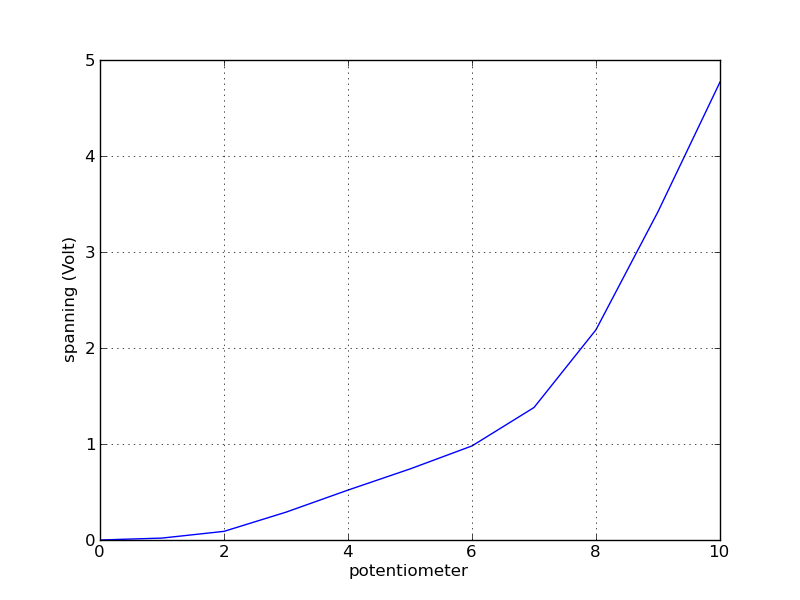
\includegraphics[width=12cm]{plot.png}
\caption{Values of the potentiometer compared the corresponding voltage.}
\end{figure}

\newpage
\addtolength{\oddsidemargin}{-1in}
\addtolength{\evensidemargin}{-1in}
\begin{figure}[H]
\caption{Diagram set-up SAR}
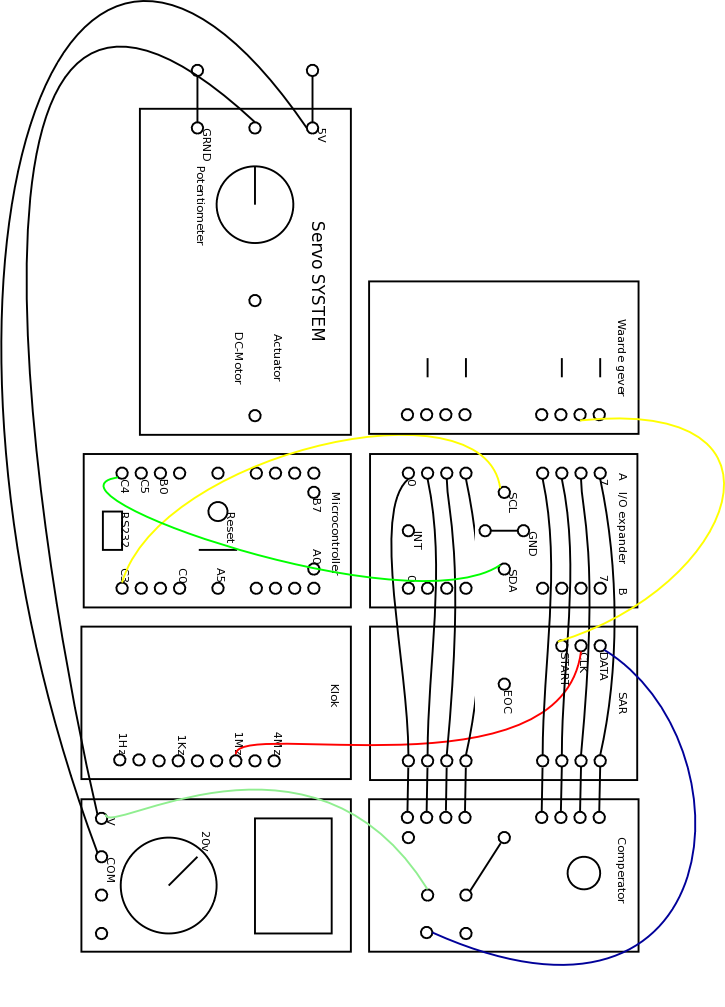
\includegraphics[scale=0.61]{SAR.png}
\end{figure}
\addtolength{\oddsidemargin}{+1in}
\addtolength{\evensidemargin}{+1in}
\newpage
% }}}
\subsection{Assumptions} % {{{
Our assumption turned out the be almost right. After doing some tests we found out that especially with a higher voltage, the relation is 0.40v/bit.

% }}}


% }}}
\newpage
\section{Servo System} % {{{

\subsection{Objective} % {{{
Our objective is to build a system that controls the position of a servo. The system also needs to detect errors (when the servo didn't reach its destination due to some reason) and needed a abort button. \\
\\
Doing this assignment will learn us how to handle and program hardware and information coming from hardware. \\
\\
We also started working on a GUI that controls the servo, but due to lack of time we weren't able to finish this.
% }}}

\subsection{Method} % {{{
We first start by modifying the setup of the previous assingment. We need a Pidac module to power the server and we need to add the microcontroller to control the system. We hook up the Pidac module to the servo and the microcontroller to the Pidac module. The microcontroller also needs to be connected to the I/O expander via a $I^{2}C$ bus and it needs to be connected to the start port of the SAR. We use a word generator to control to which position the servo needs to go and to put the Pidac module and the servo on and off. \\
\\
After taking care of the harware bit, we program the microcontroller to receive a wanted position and the current position and to turn the servo in a way that the servo will reach the wanted position.
% }}}

\subsection{Equipment} % {{{

\subsubsection{Hardware}

\begin{itemize}
\item PCF8574 I$^2$C I/O expander integrated circuit (IC).
\item Pulse generator (clock). We used one wich had different frequencies, but we liked using the 1Mhz clock.
\item SAR (successi­ve approxima­ti­on register). A SAR is a IC that conducts succesive approximation using a comperator.
\item Comperator. The comperator also has a digital to analog converter on board. The SAR gives a digital signal to the comperator and the comperator produces a currancy. This currancy is compared to the currancy on the input of the comperator. If the analog input currancy is higher than the produced currancy, the comperator will return a 1 to the SAR. Otherwise, a 0.
\item Potentiometer. On the potentiometer there are 11 spots, marked from 0 to 10. On each of these spots the potentiometer will give a certain currance. This currancy will grow exponetially going from 0 to 10. 
\item Servo. A Servo that turns around the nob of the potentiometer.
\item A voltage meter. We used a voltage meter to measure the currancy coming the potentiometer. 
\item 16F876 microcontroller: this is an 8 bit microcontroller that we load with
programs written in mplab \dots
\item 74LS244 word (8 bit) generator. Buttons toggle each of the eight pins
representing the 8 bits of output.
\item L293D PIDAC-module. The Pidac module powers the servo.
\end{itemize}

\subsubsection{Software}
The follows software runs on an i86 Windows XP machine which is connected to the
microcontroller using a serial port cable.
\begin{itemize}
\item Tera Term Web 3.1 : used as a terminal console for the microcontroller.
\item MPLAB IDE v6.30
\item PIDAC 876 programmer: Loads the compiled program onto the microcontroller
using the serial port.
\end{itemize}

% }}}

\subsection{Raw results} % {{{
After implementing the hardware and programming the micocontroller, the servo was able to stop on 4 given positions and give an error when the motor got stuck.
% }}}

\subsection{Results} % {{{

The function to let the motor stop on 4 positions is implemented.

\newpage
\addtolength{\oddsidemargin}{-1in}
\addtolength{\evensidemargin}{-1in}
\begin{figure}[H]
\caption{Diagram set-up Servo SYSTEM}
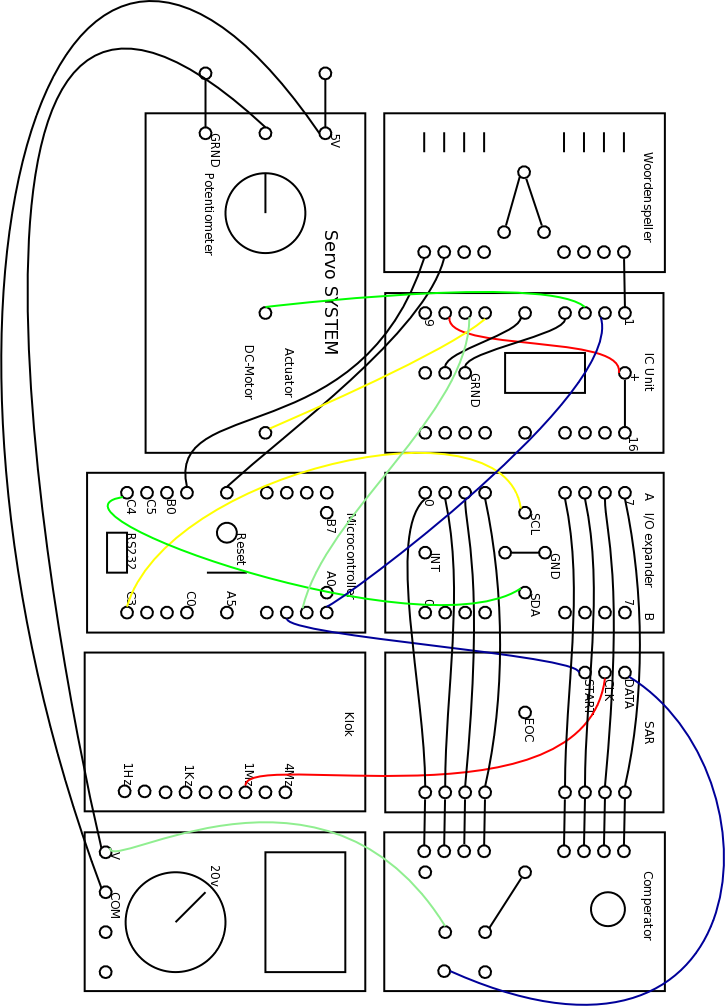
\includegraphics[scale=0.45]{Servo.png}
\end{figure}

\addtolength{\oddsidemargin}{+1in}
\addtolength{\evensidemargin}{+1in}
\newpage
\begin{figure}[H]
\caption{Part one of setup}
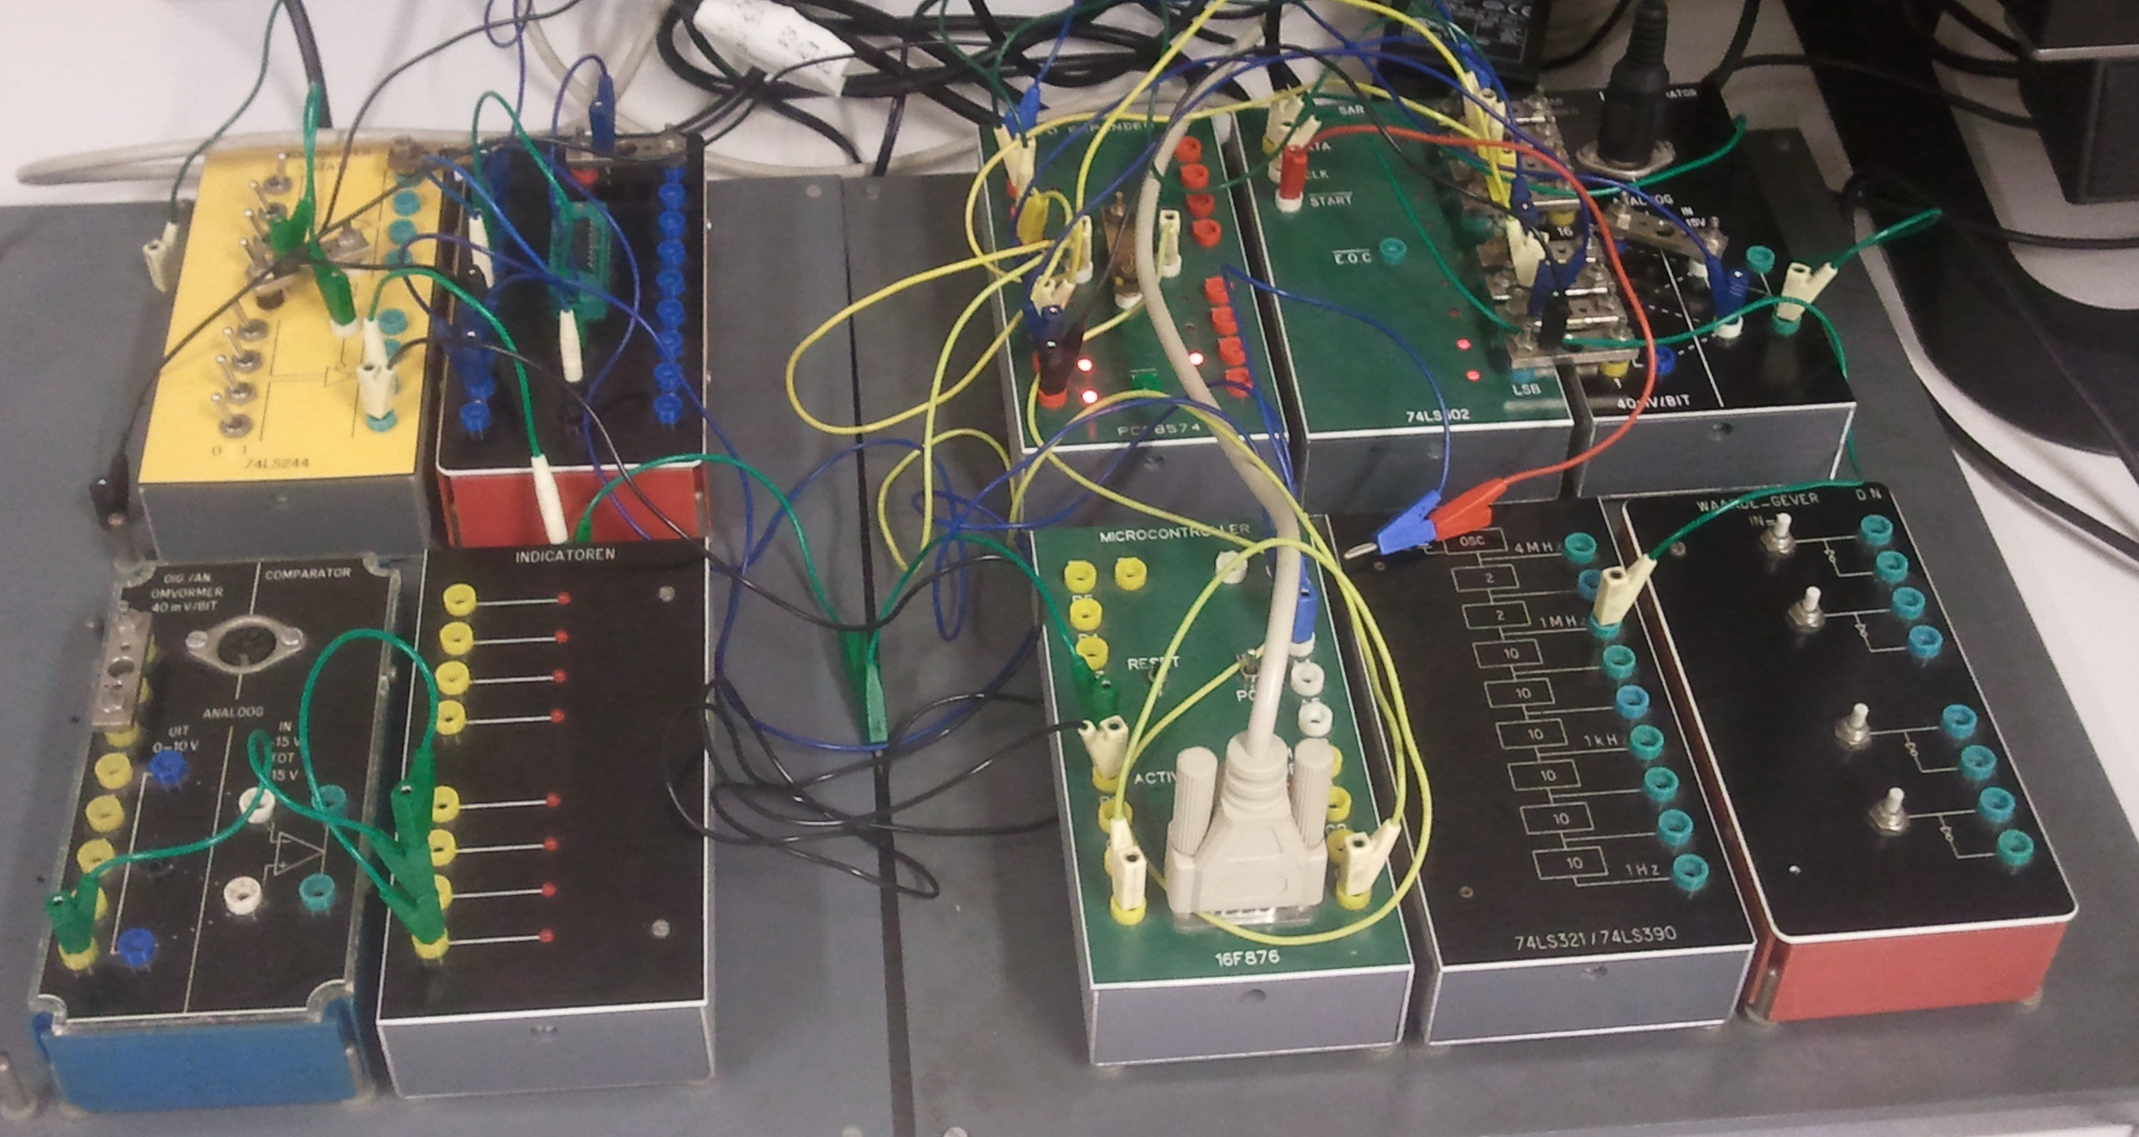
\includegraphics[scale=0.20]{servo_01.jpg}
\end{figure}
\begin{figure}[H]
\caption{Part two of setup}
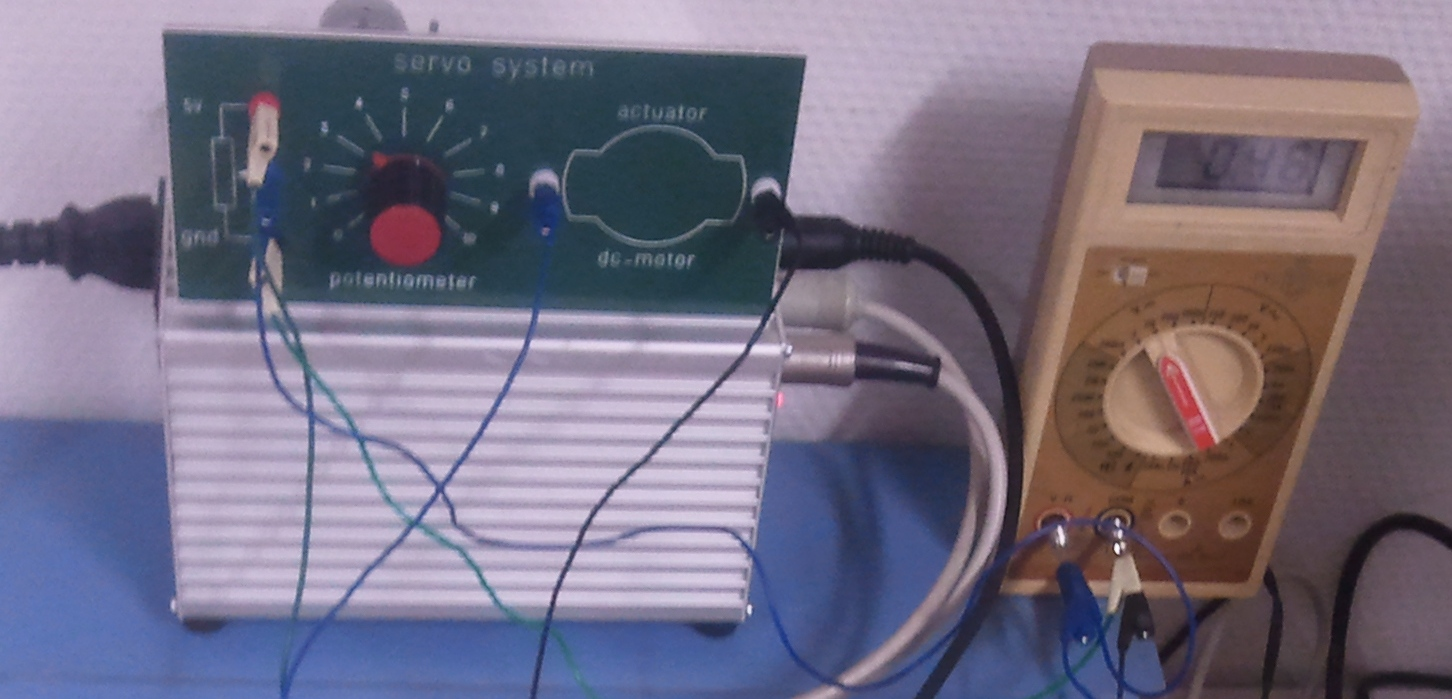
\includegraphics[scale=0.20]{servo_02.jpg}
\end{figure}
% }}}

\subsection{Assumptions} % {{{
There were no assumptions.
% }}}

% }}}

\newpage
\appendix
\addtolength{\oddsidemargin}{-1in}
\addtolength{\evensidemargin}{-1in}
\section{Source: I$^2$C} % {{{

\lstset{language=C}
\lstinputlisting{I2C.c}
% }}}

\newpage
\section{Source: Servo System} % {{{
\lstset{language=C}
\lstinputlisting{Servo.c}

\end{document}
